\documentclass{article}

\usepackage{tikz} 
% Added arrows.meta for cleaner arrowheads
\usetikzlibrary{automata, positioning, arrows, arrows.meta} 

\usepackage{amsthm}
\usepackage{amsfonts}
\usepackage{amsmath}
\usepackage{amssymb}
\usepackage{fullpage}
\usepackage{color}
\usepackage{parskip}
\usepackage{hyperref}
  \hypersetup{
    colorlinks = true,
    urlcolor = blue,       % color of external links using \href
    linkcolor= blue,       % color of internal links 
    citecolor= blue,       % color of links to bibliography
    filecolor= blue,        % color of file links
    }
    
\usepackage{listings}
\usepackage[utf8]{inputenc}                                                    
\usepackage[T1]{fontenc}                                                       

\definecolor{dkgreen}{rgb}{0,0.6,0}
\definecolor{gray}{rgb}{0.5,0.5,0.5}
\definecolor{mauve}{rgb}{0.58,0,0.82}

\lstset{frame=tb,
  language=haskell,
  aboveskip=3mm,
  belowskip=3mm,
  showstringspaces=false,
  columns=flexible,
  basicstyle={\small\ttfamily},
  numbers=none,
  numberstyle=\tiny\color{gray},
  keywordstyle=\color{blue},
  commentstyle=\color{dkgreen},
  stringstyle=\color{mauve},
  breaklines=true,
  breakatwhitespace=true,
  tabsize=3
}

\newtheoremstyle{theorem}
  {\topsep}   % ABOVESPACE
  {\topsep}   % BELOWSPACE
  {\itshape\/}  % BODYFONT
  {0pt}       % INDENT (empty value is the same as 0pt)
  {\bfseries} % HEADFONT
  {.}         % HEADPUNCT
  {5pt plus 1pt minus 1pt} % HEADSPACE
  {}          % CUSTOM-HEAD-SPEC
\theoremstyle{theorem} 
   \newtheorem{theorem}{Theorem}[section]
   \newtheorem{corollary}[theorem]{Corollary}
   \newtheorem{lemma}[theorem]{Lemma}
   \newtheorem{proposition}[theorem]{Proposition}
\theoremstyle{definition}
   \newtheorem{definition}[theorem]{Definition}
   \newtheorem{example}[theorem]{Example}
\theoremstyle{remark}    
  \newtheorem{remark}[theorem]{Remark}

% ==========================================
% Global TikZ Settings for Automata Diagrams
% ==========================================
\tikzset{
    ->, % Directed edges
    >=stealth, % Nice arrowheads
    node distance=3cm, % Standard distance between nodes
    every state/.style={thick, fill=gray!10}, % Styling for states
    initial text=$ $, % Removes the "start" text on the initial arrow
}

\title{CPSC-406 Report}
\author{Farzana Chowdhury  \\ Chapman University}

\date{\today} 

\begin{document}

\maketitle

\begin{abstract}
\end{abstract}

\setcounter{tocdepth}{3}
\tableofcontents
\newpage

\section{Introduction}\label{intro}

\section{Week by Week}\label{homework}

\subsection{Week 1}

\subsubsection{DFAs}

\textbf{Exercise 1}

\textbf{1. Which of the following words are accepted/refused by $\mathcal{A}_1$ and $\mathcal{A}_2$? Complete the table.}

\begin{center}
\renewcommand{\arraystretch}{1.5}
\begin{tabular}{|c|c|c|}
\hline
\textbf:{$w$} & \textbf{accepted by $\mathcal{A}_1$?} & \textbf{accepted by $\mathcal{A}_2$?} \\
\hline
$aaa$ & $\times$ & \checkmark \\
\hline
$aab$ & \checkmark & $\times$ \\
\hline
$aba$ & $\times$ & $\times$ \\
\hline
$abb$ & $\times$ & $\times$ \\
\hline
$baa$ & $\times$ & \checkmark \\
\hline
$bab$ & $\times$ & $\times$ \\
\hline
$bba$ & $\times$ & $\times$ \\
\hline
$bbb$ & $\times$ & $\times$ \\
\hline
\end{tabular}
\end{center}

\vspace{0.5cm}
\textbf{2. More generally, can you completely describe the languages $L(\mathcal{A}_k)$ accepted by $\mathcal{A}_k$, for $k=1, 2$?}

\begin{itemize}
	\item $L(\mathcal{A}_1)$: The language of all words over $\{a, b\}$ that start with the letter $a$ and end with an odd number of consecutive $b$'s. 
        
    \item $L(\mathcal{A}_2)$: The language of all words over $\{a, b\}$ that end with the substring $aa$. 
    
\end{itemize}

\vspace{0.5cm}

\textbf{Exercise 2}

\textbf{Design DFAs whose accepted languages are given as follows:}

% ---------------------------------------------------------
\vspace{0.5cm}
\textbf{1. All the words that end with $ab$}

\begin{center}
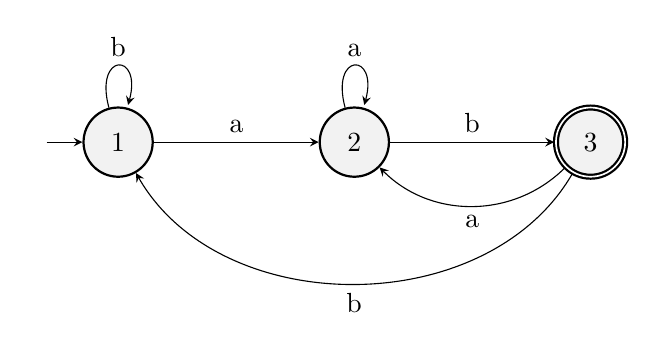
\begin{tikzpicture}
    \node[state, initial] (q1) {1};
    \node[state] (q2) [right of=q1] {2};
    \node[state, accepting] (q3) [right of=q2] {3};

    \path
        (q1) edge [loop above] node {b} (q1)
             edge node[above] {a} (q2)
        (q2) edge [loop above] node {a} (q2)
             edge node[above] {b} (q3)
        (q3) edge [bend left=45] node[below] {a} (q2)
             edge [bend left=60] node[below] {b} (q1);
\end{tikzpicture}
\end{center}

% ---------------------------------------------------------
\vspace{0.5cm}
\textbf{2. All the words that contain $aba$}

\begin{center}
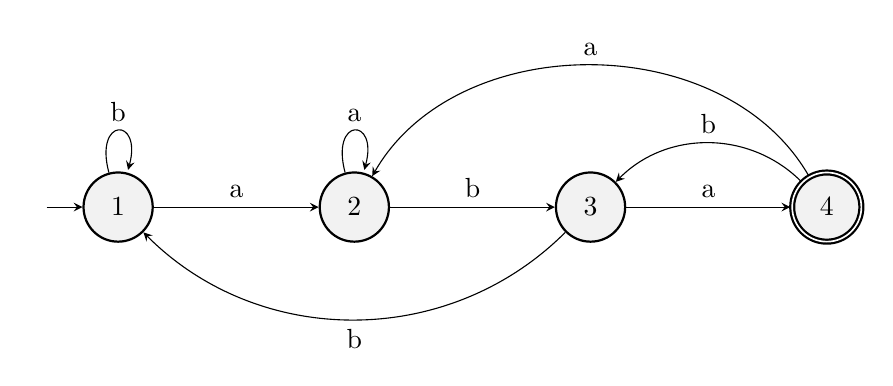
\begin{tikzpicture}
    \node[state, initial] (q1) {1};
    \node[state] (q2) [right of=q1] {2};
    \node[state] (q3) [right of=q2] {3};
    \node[state, accepting] (q4) [right of=q3] {4};

    \path
        (q1) edge [loop above] node {b} (q1)
             edge node[above] {a} (q2)
        (q2) edge [loop above] node {a} (q2)
             edge node[above] {b} (q3)
        (q3) edge [bend left=45] node[below] {b} (q1)
             edge node[above] {a} (q4)
        (q4) edge [bend right=60] node[above] {a} (q2)
             edge [bend right=45] node[above] {b} (q3);
\end{tikzpicture}
\end{center}

% ---------------------------------------------------------
\vspace{0.5cm}
\textbf{3. All the words that contain an odd number of $a$'s and an odd number of $b$'s}

\begin{center}
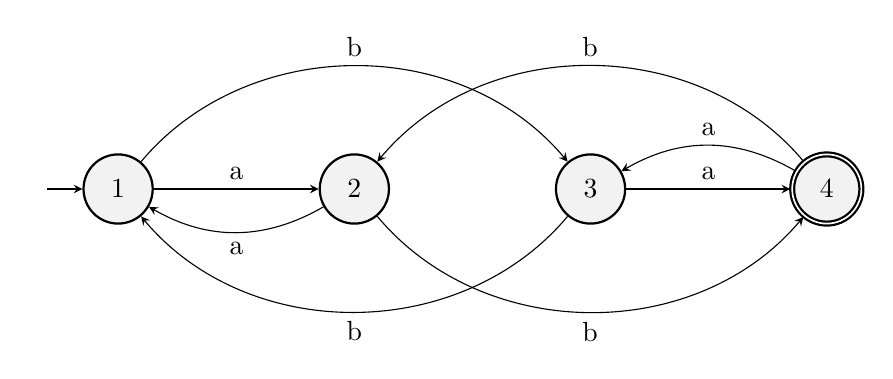
\begin{tikzpicture}
    \node[state, initial] (q1) {1};
    \node[state] (q2) [right of=q1] {2};
    \node[state] (q3) [right of=q2] {3};
    \node[state, accepting] (q4) [right of=q3] {4};

    \path
        (q1) edge node[above] {a} (q2)
             edge [bend left=50] node[above] {b} (q3)
        (q2) edge [bend left] node[below] {a} (q1)
             edge [bend right=50] node[below] {b} (q4)
        (q3) edge [bend left=50] node[below] {b} (q1)
             edge node[above] {a} (q4)
        (q4) edge [bend right=50] node[above] {b} (q2)
             edge [bend right] node[above] {a} (q3);
\end{tikzpicture}
\end{center}

% ---------------------------------------------------------
\vspace{0.5cm}
\textbf{4. All the words that contain an even number of $a$'s and an odd number of $b$'s}

\begin{center}
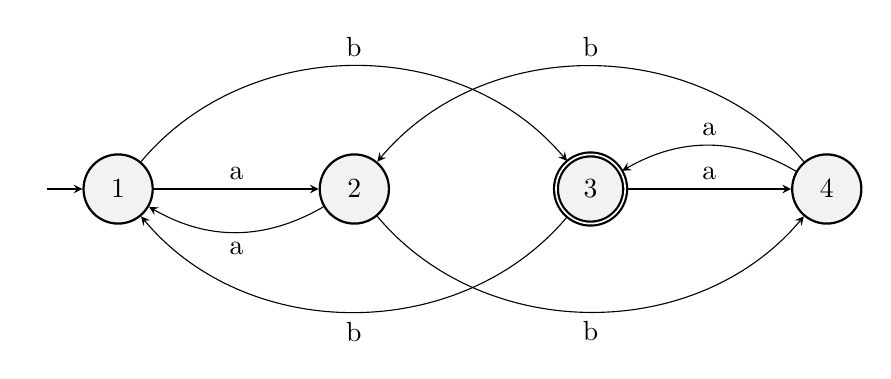
\begin{tikzpicture}
    \node[state, initial] (q1) {1};
    \node[state] (q2) [right of=q1] {2};
    \node[state, accepting] (q3) [right of=q2] {3};
    \node[state] (q4) [right of=q3] {4};

    \path
        (q1) edge node[above] {a} (q2)
             edge [bend left=50] node[above] {b} (q3)
        (q2) edge [bend left] node[below] {a} (q1)
             edge [bend right=50] node[below] {b} (q4)
        (q3) edge [bend left=50] node[below] {b} (q1)
             edge node[above] {a} (q4)
        (q4) edge [bend right=50] node[above] {b} (q2)
             edge [bend right] node[above] {a} (q3);
\end{tikzpicture}
\end{center}

% ---------------------------------------------------------
\vspace{0.5cm}
\textbf{5. All the words such that any three consecutive characters contain at least one $a$}

\begin{center}
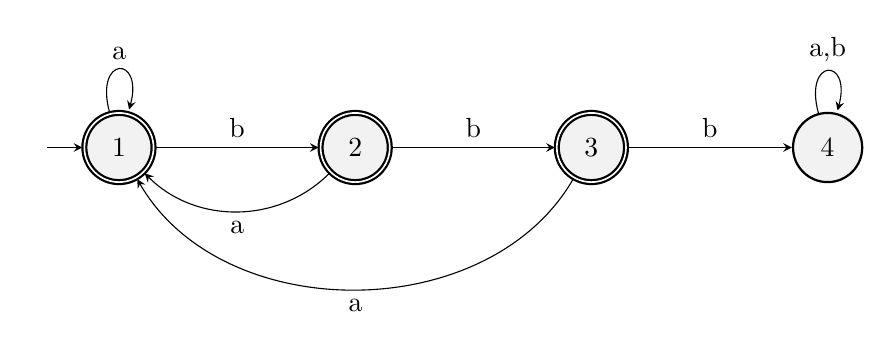
\begin{tikzpicture}
    \node[state, initial, accepting] (q1) {1};
    \node[state, accepting] (q2) [right of=q1] {2};
    \node[state, accepting] (q3) [right of=q2] {3};
    \node[state] (q4) [right of=q3] {4};

    \path
        (q1) edge [loop above] node {a} (q1)
             edge node[above] {b} (q2)
        (q2) edge [bend left=45] node[below] {a} (q1)
             edge node[above] {b} (q3)
        (q3) edge [bend left=60] node[below] {a} (q1)
             edge node[above] {b} (q4)
        (q4) edge [loop above] node {a,b} (q4);
\end{tikzpicture}
\end{center}

% ---------------------------------------------------------
\vspace{0.5cm}
\textbf{6. All the words that contain $bbb$}

\begin{center}
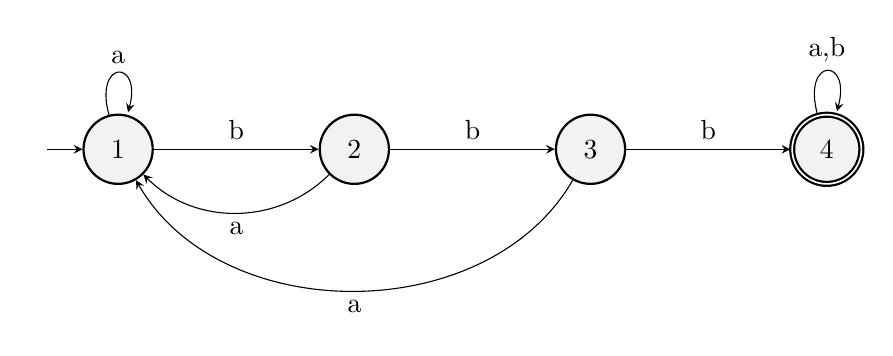
\begin{tikzpicture}
    \node[state, initial] (q1) {1};
    \node[state] (q2) [right of=q1] {2};
    \node[state] (q3) [right of=q2] {3};
    \node[state, accepting] (q4) [right of=q3] {4};

    \path
        (q1) edge [loop above] node {a} (q1)
             edge node[above] {b} (q2)
        (q2) edge [bend left=45] node[below] {a} (q1)
             edge node[above] {b} (q3)
        (q3) edge [bend left=60] node[below] {a} (q1)
             edge node[above] {b} (q4)
        (q4) edge [loop above] node {a,b} (q4);
\end{tikzpicture}
\end{center}

\textbf{What do you notice when comparing the various automata?}

For DFAs that have criteria of "ends with," arrows must leave the accept state because the string could keep going and fail to satisfy DFA characteristics. For DFAs that have criteria of , "contains," the accept state must be a "Trap State" with a self-loop, because once you find the sequence, you can traverse through the DFA while satisfying DFA's accepted language conditions.

\subsubsection{Question}
What is the easiest and best way to implement DFAs in programming?

\subsection{Week 2}

\subsubsection{Operations on automata}

\textbf{Exercise 1}
\begin{enumerate}
  \item $L(\mathcal{A}^{(1)})$ can't have $aa$ or $bb$ (two of the same letters in a row). For $L(\mathcal{A}^{(1)})$, any $a$ has to be in an odd numbered state position.
  \item
  \begin{center}
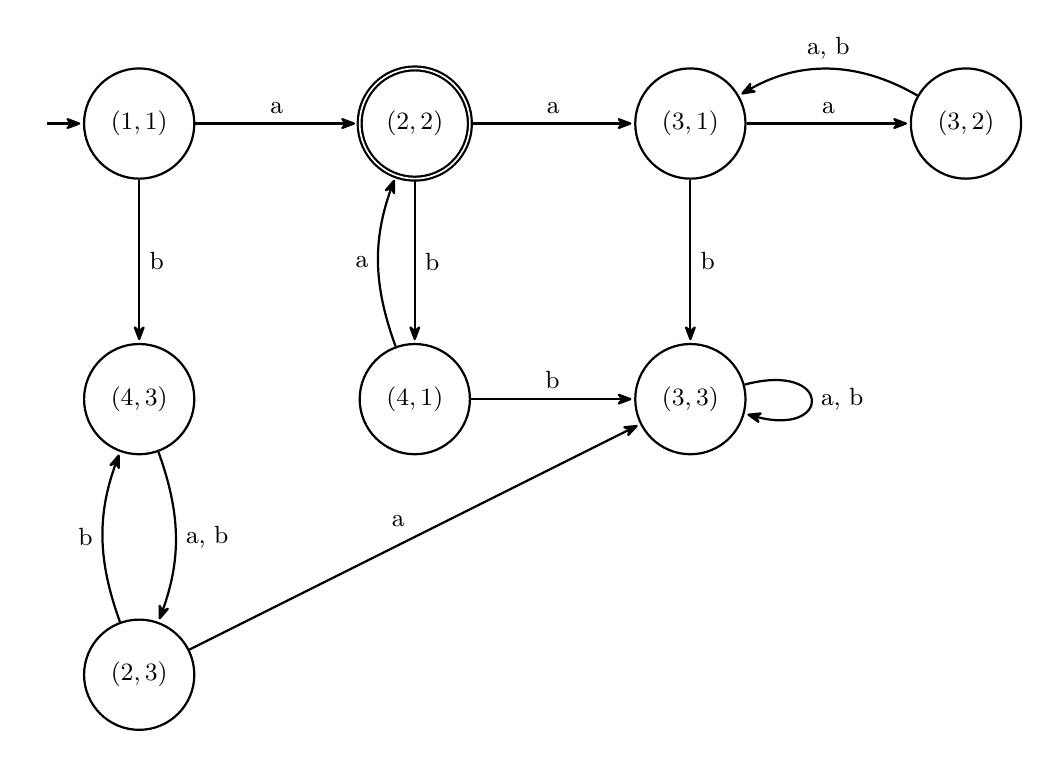
\begin{tikzpicture}[
    shorten >=1pt, node distance=3.5cm, on grid, auto, 
    thick, initial text={}, 
    every state/.style={minimum size=1.4cm, font=\small},
    >={Stealth[round]},
    every node/.style={font=\small}
]

    % --- States ---
    \node[state, initial] (s11) {$(1,1)$};
    \node[state, accepting] (s22) [right=of s11] {$(2,2)$};
    \node[state] (s31) [right=of s22] {$(3,1)$};
    \node[state] (s32) [right=of s31] {$(3,2)$};
    
    \node[state] (s43) [below=of s11] {$(4,3)$};
    \node[state] (s41) [below=of s22] {$(4,1)$};
    \node[state] (s33) [below=of s31] {$(3,3)$};
    
    \node[state] (s23) [below=of s43] {$(2,3)$};

    % --- Transitions ---
    \path[->] 
        % Row 1
        (s11) edge node {a} (s22)          % Removed extra a
              edge node {b} (s43)
        
        (s22) edge node {a} (s31)          % Removed extra a
              edge node {b} (s41)
              
        (s31) edge node {a} (s32)
              edge node {b} (s33)
        
        (s32) edge [bend right=30] node[above] {a, b} (s31)
        
        % Row 2
        (s41) edge [bend left=20] node {a} (s22)
              edge node {b} (s33)          % Removed extra a
              
        (s43) edge [bend left=20] node {a, b} (s23)
        
        (s33) edge [loop right] node {a, b} (s33)
        
        % Row 3
        (s23) edge [bend left=20] node {b} (s43)
              edge node {a} (s33);         % Removed extra a

\end{tikzpicture}
\end{center}
  \item To find the intersection of two languages ($L_1 \cap L_2$), you create a new machine that simulates how $\mathcal{A}^{(1)}$ and $\mathcal{A}^{(2)}$ work at the same time. When you take in an input $a$ or $b$, both numbers in the pair update at the same time based on their original rules. For intersection ($\cap$), you only have a double circle if both machines are in an accepting state.
  \item For union ($\cup$), you have a double circle if at least one of the machines is in an accepting state.
\end{enumerate}   

\textbf{Exercise 2}
\begin{enumerate}
    \item For $L(\mathcal{B}^{(1)})$, the total number of $a$ is a multiple of 3, including zero. For $L(\mathcal{B}^{(2)})$, every $a$ is directly followed by at least one $b$, and the string must not end with $a$. 
    \item 
    %\begin{center}
\begin{tikzpicture}[
    shorten >=1pt, 
    node distance=2.4cm, % Optimized for standard page width
    on grid, 
    auto, 
    thick, 
    initial text={}, 
    every state/.style={minimum size=1.1cm, font=\scriptsize},
    >={Stealth[round]},
    every node/.style={font=\scriptsize}
]

    % --- States ---
    \node[state, initial, accepting] (p0q0) {$(p_0, q_0)$};
    \node[state] (p1q1) [right=of p0q0] {$(p_1, q_1)$};
    \node[state] (p1q0) [right=of p1q1] {$(p_1, q_0)$};
    
    \node[state] (p0q2) [below=of p0q0] {$(p_0, q_2)$};
    \node[state] (p2q2) [below=of p1q1] {$(p_2, q_2)$};
    \node[state] (p2q1) [below=of p1q0] {$(p_2, q_1)$};
    
    \node[state] (p1q2) [below=of p0q2] {$(p_1, q_2)$};
    \node[state] (p2q0) [below=of p2q1] {$(p_2, q_0)$};
    
    \node[state] (p0q1) [below=of p2q0] {$(p_0, q_1)$};

    % --- Transitions ---
    \path[->] 
        % Row 1
        (p0q0) edge [loop above] node {b} (p0q0)
               edge node {a} (p1q1)
               edge node[left] {a} (p0q2)
        (p1q1) edge node {b} (p1q0)
               edge node[left] {a} (p2q2)
        (p1q0) edge [loop above] node {b} (p1q0)
               edge node {a} (p2q1)
        
        % Row 2
        (p0q2) edge [loop left] node {b} (p0q2)
               edge node[swap] {a} (p1q2) 
        (p2q2) edge [loop right] node {b} (p2q2)
               edge [bend left=15] node {a} (p0q2)
        
        % RE-ROUTED: p2q1 to p0q2 (Underneath Row 2)
        % This bend and looseness avoids p2q2, p1q1, and p1q0 entirely.
        (p2q1) edge node {b} (p2q0)
               edge [bend left=40, looseness=1.2] node[below, pos=0.5] {a} (p0q2)
        
        % Row 3
        (p1q2) edge [loop left] node {b} (p1q2)
               edge node[above, pos=0.6] {a} (p2q2)
        (p2q0) edge [loop right] node {b} (p2q0)
               edge node {a} (p0q1)

        % THE LONG RETURN (Avoids Left Margin Cutoff)
        (p0q1) edge [bend left=110, looseness=2.5] node[left, pos=0.4] {b} (p0q0)
               edge [bend left=25] node[right] {a} (p1q2);

\end{tikzpicture}
%\end{center}
\item Since the only accepting state is $(p_0, q_0)$, a string is accepted if and only if it leads both $L(\mathcal{B}^{(1)})$ and $L(\mathcal{B}^{(2)})$ to an accepting state.  
    \item A state will be accepting if the first part is $p_0$ or if the second part is not $q_0$.
\end{enumerate}   

\textbf{Exercise 2.2.7}
\textbf{Basis:} \\
Let the length of the string be $n=0$. The empty string, $\epsilon$, is of length 0.
\[ \hat{\delta}(q, \epsilon) = q \]
$\therefore$ The basis is true.

\vspace{1em}

\textbf{Inductive Hypothesis:} \\
Assume that for any string $w$ of length $n$, $\hat{\delta}(q, w) = q$.

\vspace{1em}

\textbf{Inductive Step:} \\
Consider a string $x$ of length $n+1$. The string can be written as $x = wa$, where $w$ is a string of length $n$ and $a$ is a single input symbol ($a \in \Sigma$).

\begin{align*}
\hat{\delta}(q, wa) &= \delta(\hat{\delta}(q, w), a) && \text{-- by definition of } \hat{\delta} \\
&= \delta(q, a) && \text{-- by Inductive Hypothesis: } \hat{\delta}(q, w) = q \\
&= q && \text{-- by given property: } \delta(q, a) = q \text{ for all } a
\end{align*}

\subsubsection{Question}
What other mathematical properties aside from intersection and union could be applied to automata?
\section{Synthesis}

\section{Evidence of Participation}

\section{Conclusion}\label{conclusion}

\begin{thebibliography}{99}
\bibitem[BLA]{bla} Author, \href{https://en.wikipedia.org/wiki/LaTeX}{Title}, Publisher, Year.
\end{thebibliography}

\end{document}
